\input{"../../../preamble"}

\begin{document}

\title{CSC263-Notes-01-26-2015}

\input{"../csc263-header"}
\rhead{January 26, 2015}

\section*{Lecture 07}

\subsection*{AVL Trees}

\begin{center}
\begin{tabular}{c c c}

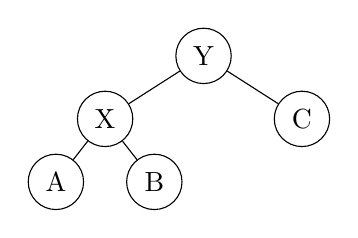
\begin{tikzpicture}[every node/.style={circle,draw,minimum size=2em,inner sep=1},
	baseline={(current bounding box.center)},
	level/.style={level distance=8mm,
	sibling distance=25mm/#1}]
\node {Y} 
child {node {X}
	child {node {A}}
	child {node {B}}
	}
child {node {C}};
\end{tikzpicture} &

\pbox{10cm}{
	right rotation $\rightarrow$ \\
	$\leftarrow$ left rotation
} &

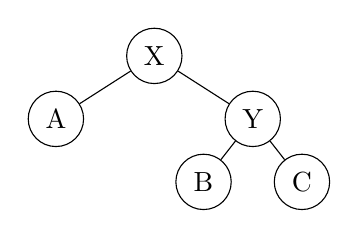
\begin{tikzpicture}[every node/.style={circle,draw,minimum size=2em,inner sep=1},
	baseline={(current bounding box.center)},
	level/.style={level distance=8mm,
	sibling distance=25mm/#1}]
\node {X} 
child {node {A}}
child {node {Y}
	child {node {B}}
	child {node {C}}
	};
\end{tikzpicture} \\

\end{tabular}
\end{center}

\begin{itemize}
 	\item Three references to change: parent's left/right, y.left, x.right
 	\item Decreases depth of subtree $A$, increases depth of subtree $C$
\end{itemize} 

\begin{tabular}{c c c c c}

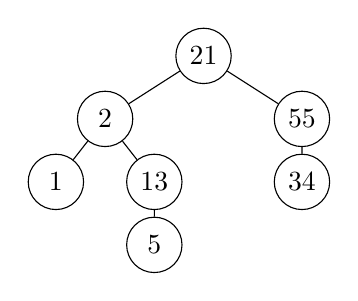
\begin{tikzpicture}[every node/.style={circle,draw,minimum size=2em,inner sep=1},
	baseline={(current bounding box.center)},
	level/.style={level distance=8mm,
	sibling distance=25mm/#1}]
\node {21} 
child {node {2}
	child { node{1}}
	child { node{13}
		child {node {5}}
		}
}
child {node {55}
	child {node {34}}
	};
\end{tikzpicture} &

insert 3 $\rightarrow$ &

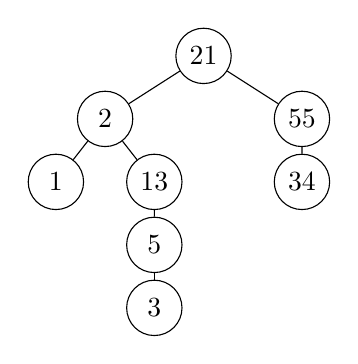
\begin{tikzpicture}[every node/.style={circle,draw,minimum size=2em,inner sep=1},
	baseline={(current bounding box.center)},
	level/.style={level distance=8mm,
	sibling distance=25mm/#1}]
\node {21} 
child {node {2}
	child { node{1}}
	child { node{13}
		child {node {5}
			child {node {3}}
			}
		}
	}
child {node {55}
	child {node {34}}
	};
\end{tikzpicture} &

\pbox{10cm}{
	right rotation $\rightarrow$ \\
	(around 5-13)
} &

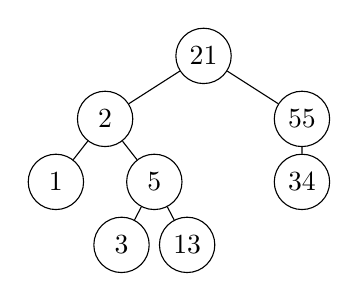
\begin{tikzpicture}[every node/.style={circle,draw,minimum size=2em,inner sep=1},
	baseline={(current bounding box.center)},
	level/.style={level distance=8mm,
	sibling distance=25mm/#1}]
\node {21} 
child {node {2}
	child { node{1}}
	child { node{5}
		child {node {3}}
		child {node {13}}
		}
}
child {node {55}
	child {node {34}}
	};
\end{tikzpicture}

\end{tabular}

\begin{itemize}
	\item computing height takes time $\Theta(s)$ where $s$ = size of subtree
	\item instead, have each node store node.height (for subtree rooted at node)
\end{itemize}

\begin{tabular}{c c c c c}

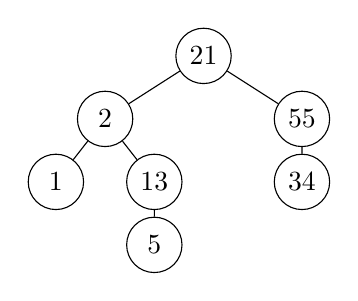
\begin{tikzpicture}[every node/.style={circle,draw,minimum size=2em,inner sep=1},
	baseline={(current bounding box.center)},
	level/.style={level distance=8mm,
	sibling distance=25mm/#1}]
\node {21} 
child {node {2}
	child { node{1}}
	child { node{13}
		child {node {5}}
		}
}
child {node {55}
	child {node {34}}
	};
\end{tikzpicture} &

insert 3 $\rightarrow$ &

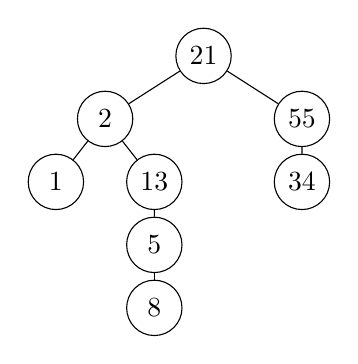
\begin{tikzpicture}[every node/.style={circle,draw,minimum size=2em,inner sep=1},
	baseline={(current bounding box.center)},
	level/.style={level distance=8mm,
	sibling distance=25mm/#1}]
\node {21}
child { node{2}
	child { node{1}}
	child { node{13}
		child { node{5}
			child { node{8}}
			}
		}
	}
child { node{55}
	child { node{34}}
	};
\end{tikzpicture} &

rotate right $\rightarrow$ &

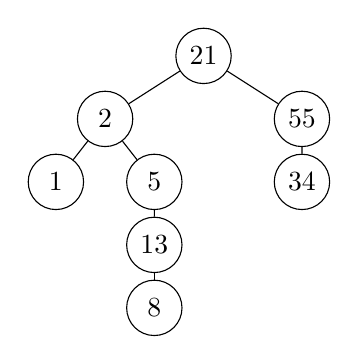
\begin{tikzpicture}[every node/.style={circle,draw,minimum size=2em,inner sep=1},
	baseline={(current bounding box.center)},
	level/.style={level distance=8mm,
	sibling distance=25mm/#1}]
\node {21}
child { node{2}
	child { node{1}}
	child { node{5}
		child { node{13}
			child { node{8}}
			}
		}
	}
child { node{55}
	child { node{34}}
	};
\end{tikzpicture}

\end{tabular} \\

\noindent Problem: rotation does not fix balance $\rightarrow$ double rotation!

\begin{tabular}{c c c c c}

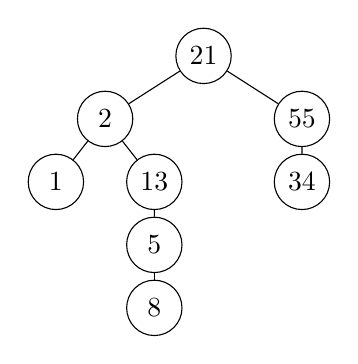
\begin{tikzpicture}[every node/.style={circle,draw,minimum size=2em,inner sep=1},
	baseline={(current bounding box.center)},
	level/.style={level distance=8mm,
	sibling distance=25mm/#1}]
\node {21}
child { node{2}
	child { node{1}}
	child { node{13}
		child { node{5}
			child { node{8}}
			}
		}
	}
child { node{55}
	child { node{34}}
	};
\end{tikzpicture} &

\pbox{10cm}{
	rotate left \\ on tree \\
	rooted at 5 $\rightarrow$
} &

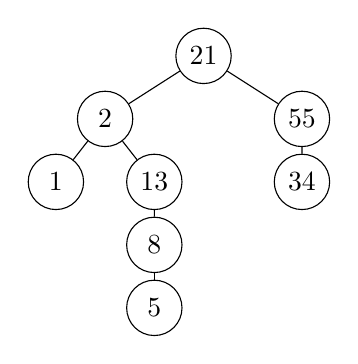
\begin{tikzpicture}[every node/.style={circle,draw,minimum size=2em,inner sep=1},
	baseline={(current bounding box.center)},
	level/.style={level distance=8mm,
	sibling distance=25mm/#1}]
\node {21}
child { node{2}
	child { node{1}}
	child { node{13}
		child { node{8}
			child { node{5}}
			}
		}
	}
child { node{55}
	child { node{34}}
	};
\end{tikzpicture} &

\pbox{10cm}{
	rotate right \\ on tree \\
	rooted at 13 $\rightarrow$
}

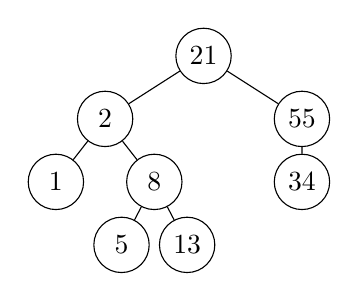
\begin{tikzpicture}[every node/.style={circle,draw,minimum size=2em,inner sep=1},
	baseline={(current bounding box.center)},
	level/.style={level distance=8mm,
	sibling distance=25mm/#1}]
\node {21}
child { node{2}
	child { node{1}}
	child { node{8}
		child { node{5}}
		child { node{13}}
		}
	}
child { node{55}
	child { node{34}}
	};
\end{tikzpicture}

\end{tabular}

\begin{tabular}{c c c}

\pbox{10cm}{
	insert 3 $\rightarrow$
} & 

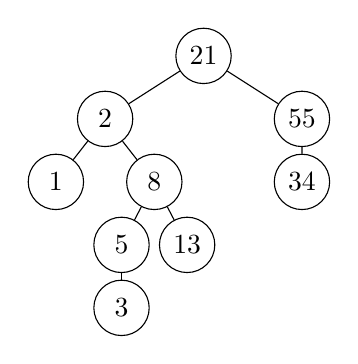
\begin{tikzpicture}[every node/.style={circle,draw,minimum size=2em,inner sep=1},
	baseline={(current bounding box.center)},
	level/.style={level distance=8mm,
	sibling distance=25mm/#1}]
\node {21}
child { node{2}
	child { node{1}}
	child { node{8}
		child { node{5}
			child { node{3}}
			}
		child { node{13}}
		}
	}
child { node{55}
	child { node{34}}
	};
\end{tikzpicture} &

\pbox{10cm}{
	$\rightarrow$ subtree rooted at 8 balanced, \\
	subtree rooted at 2 is unbalanced
}

\end{tabular}

\end{document}